\chapter{STRUC/TURE} 
\label{sec:baydoor}
\lstset{style=6502Style}

\begin{figure}[H]
    \begin{adjustbox}{width=13.2cm,left}
      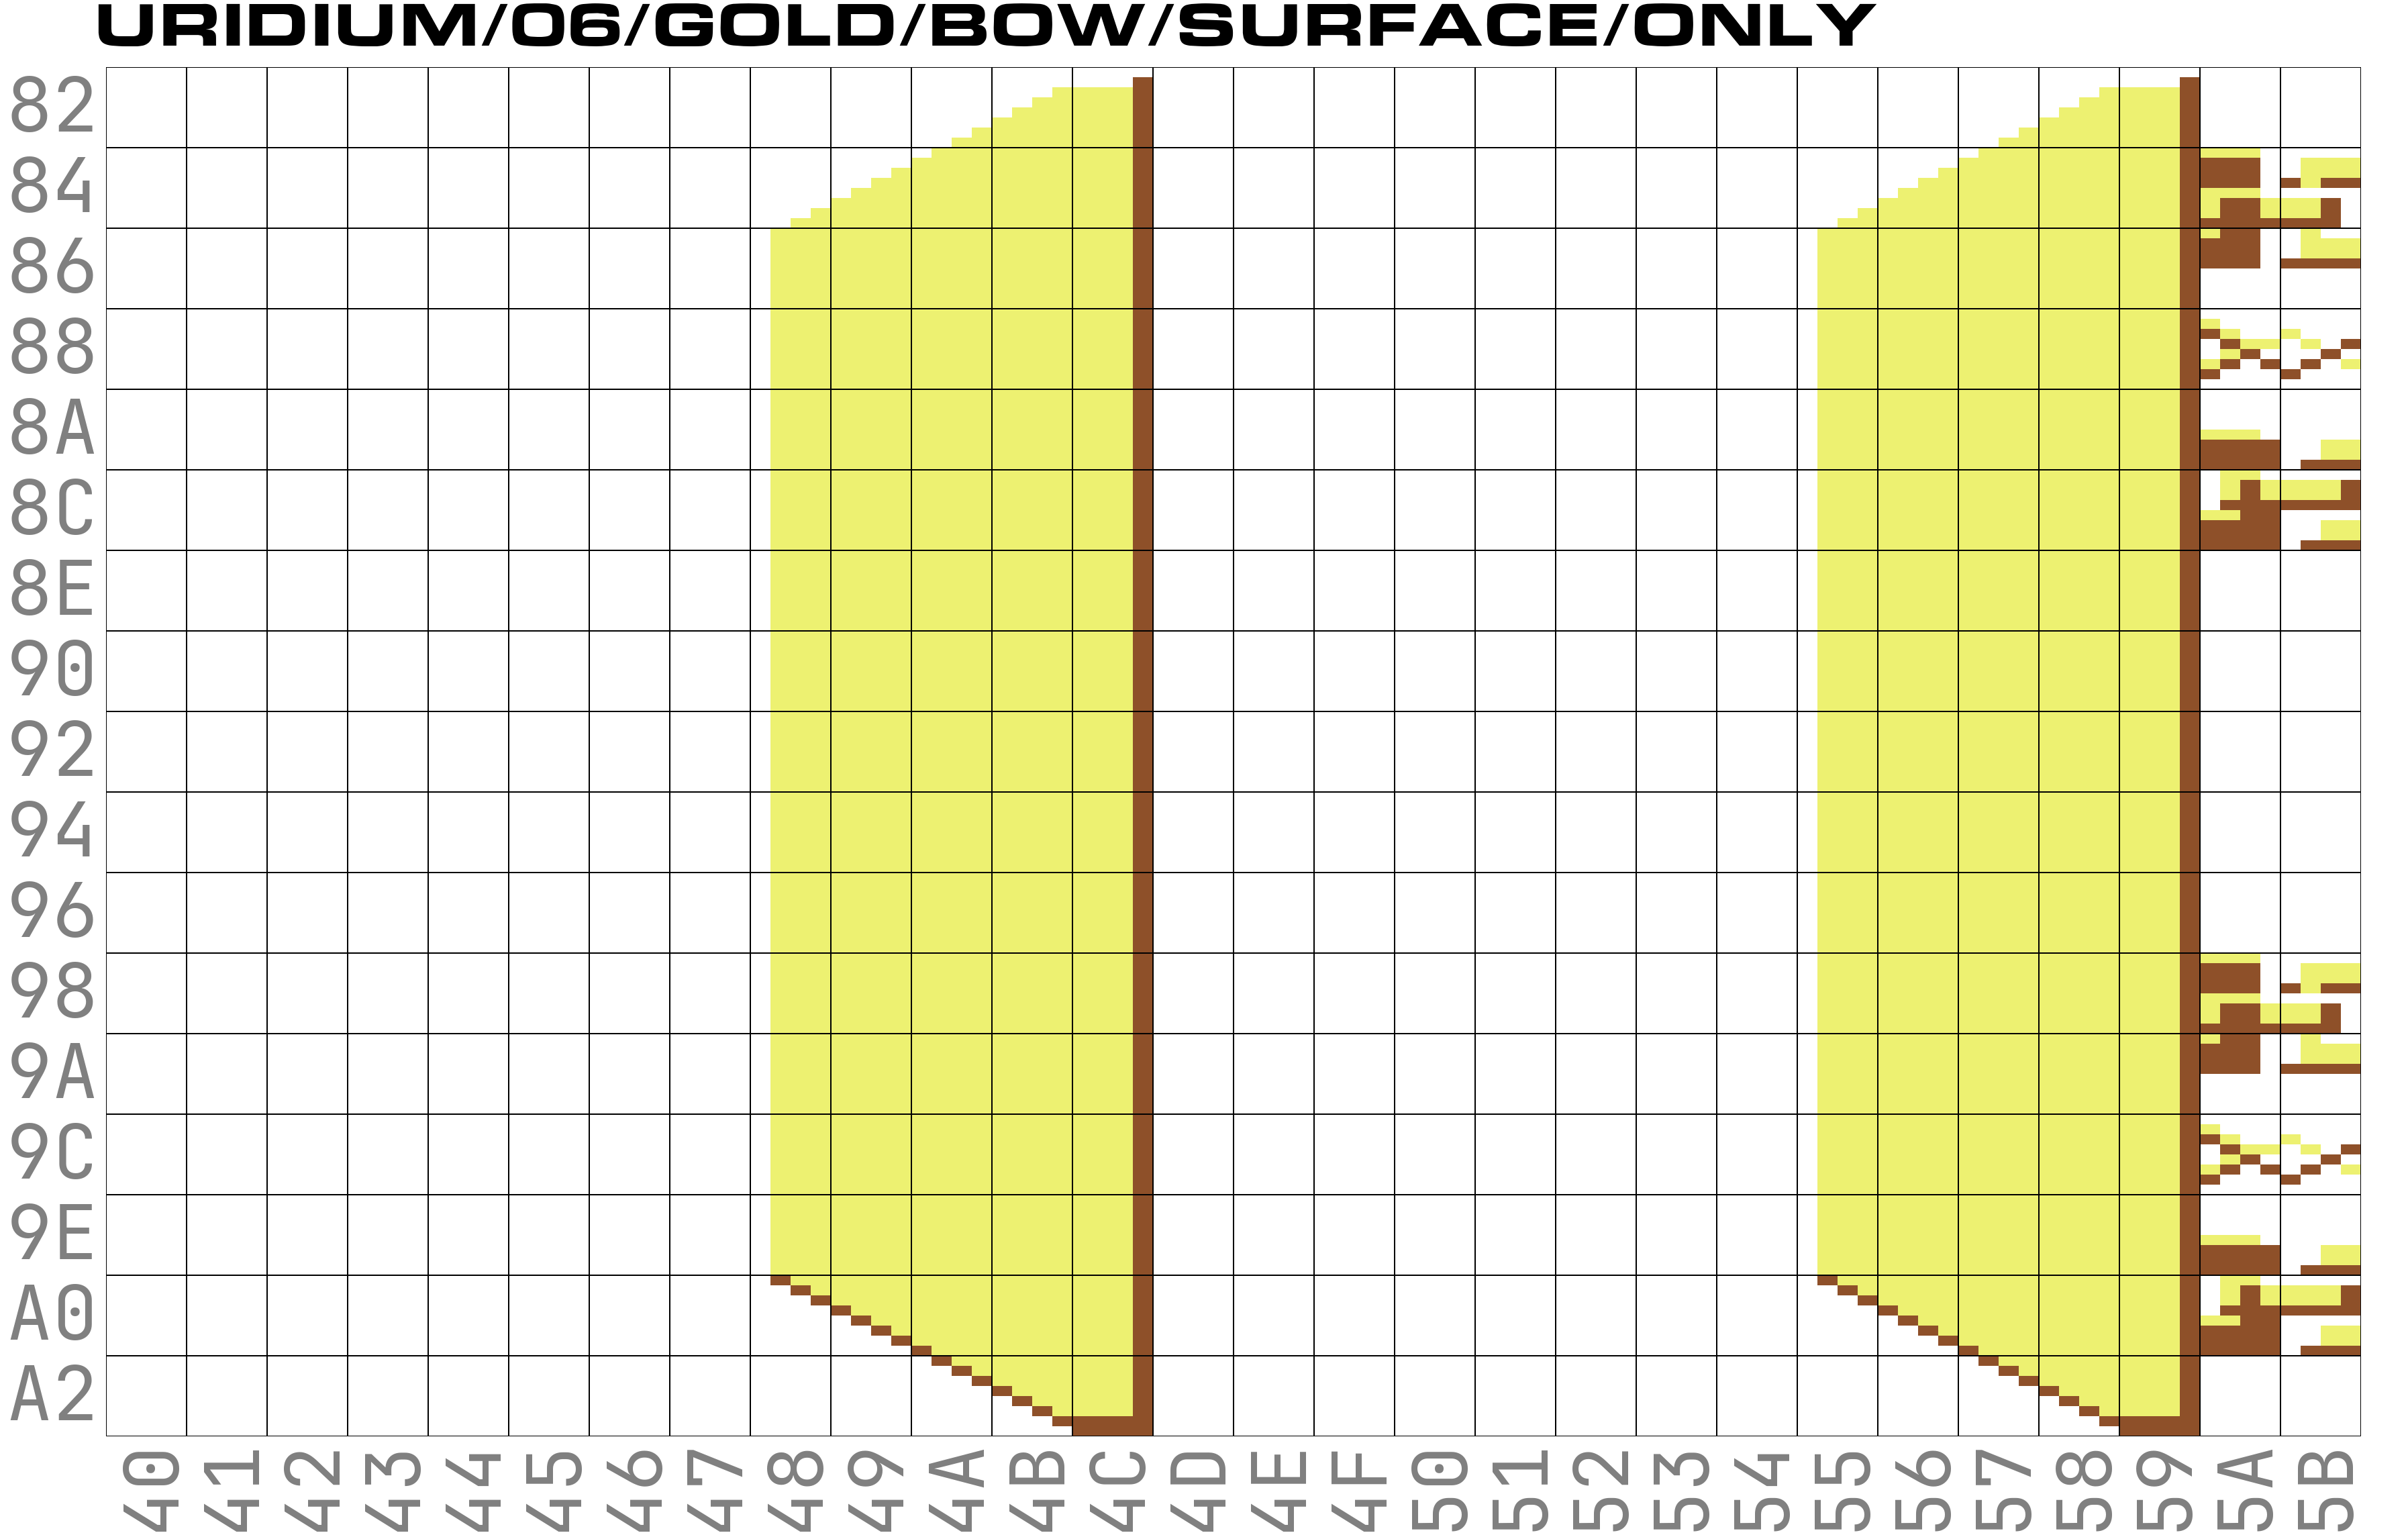
\includegraphics{src/surface_diagrams_with_sections/6_1_8B_0D_surface.png}%
    \end{adjustbox}
\end{figure}
\vspace{-0.4cm}
This is what the bow of the dreadnought in Level 6 looks like after our first pass.
It's incomplete, as we noticed. We're missing two forward sections as well as a portal
detail, among other things. What we need is a way of defining the structures that
we need to place on the surface and where to position them.

\vspace{-0.2cm}
\begin{wrapfigure}{tr}{6cm} % <==========================================
\begin{lstlisting}
.BYTE $9E ; High Byte (Row)
.BYTE $40 ; Low Byte (Col)
.BYTE $8B ; Structure to Place

.BYTE $9E ; High Byte (Row)
.BYTE $4D ; Low Byte (Col)
.BYTE $8B ; Structure to Place

.BYTE $98 ; High Byte (Row)
.BYTE $46 ; Low Byte (Col)
.BYTE $0D ; Structure to Place
\end{lstlisting}
\end{wrapfigure}
The way we go about solving this is given in the inset listing here. For each of the three
structure we want to place we define the row and the column where we want to place
it, along with a reference to the structure that we want to insert. The important
thing to notice in the way we have defined the row and column is that we have given the
bottom left position of the structure as the starting point. So when you look at row \icode{\$9E}
and column \icode{\$40} below you will notice it gives the bottom left corner of the placed 
structure.
\footnote{
  The row and column references are in fact memory addresses. So \icode{\$9E} and \icode{\$40} combine to
  give the address \icode{\$9E40}. The region of memory between \icode{\$8200} and \icode{\$A400} is
  treated as a table 17 rows tall by 512 columns wide. That is why our row references increment by 2 
  rather than 1: the first 256 columns of row 15 are between \icode{\$9E00} and \icode{\$9F00}, while
  the second 256 columns are between \icode{\$9F00} and \icode{\$A000}.
}

This method allows us to place structures arbitrarily along the surface of the dreadnought. In the
diagram below we have placed the three structures defined in our inset listing: \icode{\$0D} and
two instances of \icode{\$8B}.

\begin{figure}[H]
    \begin{adjustbox}{width=13.2cm,left}
      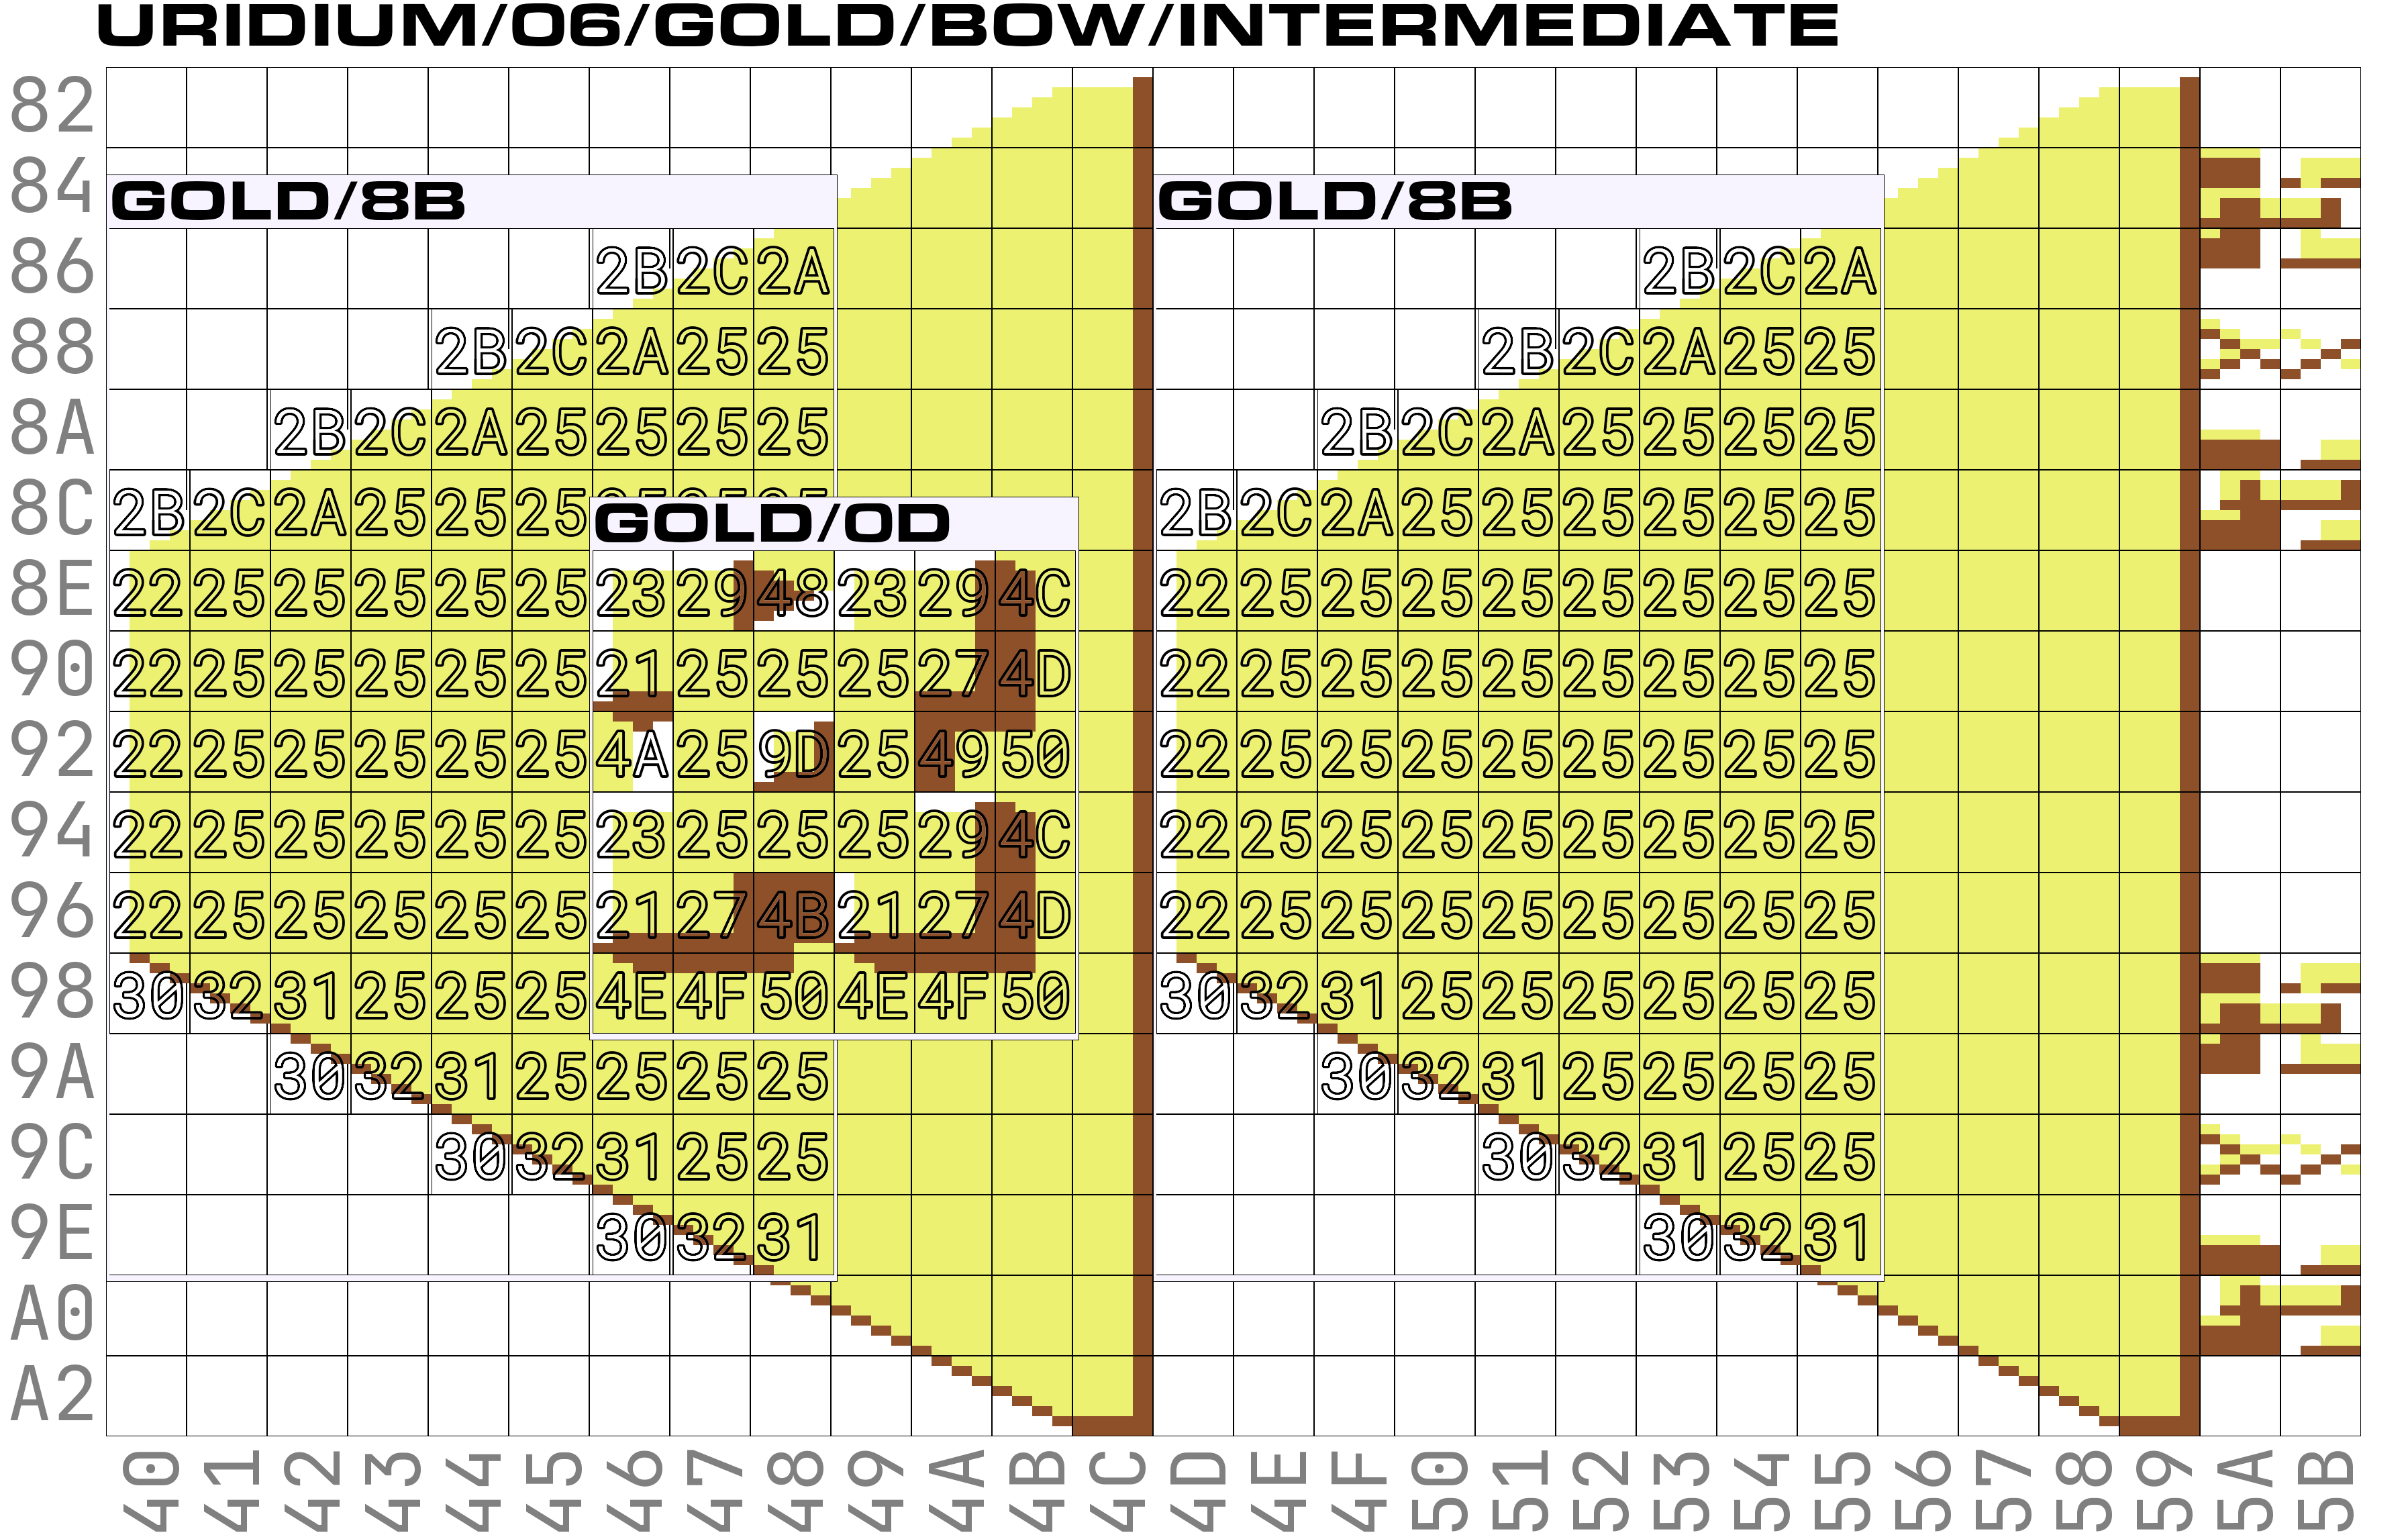
\includegraphics{src/surface_diagrams_with_sections/6_1_8B_0D.png}%
    \end{adjustbox}
\end{figure}
\vspace{-0.4cm}

Of course there are more than just three structures to place on the dreadnought. There are numerous
plinths casting many different shadows.

\raisebox{-0.1\totalheight}{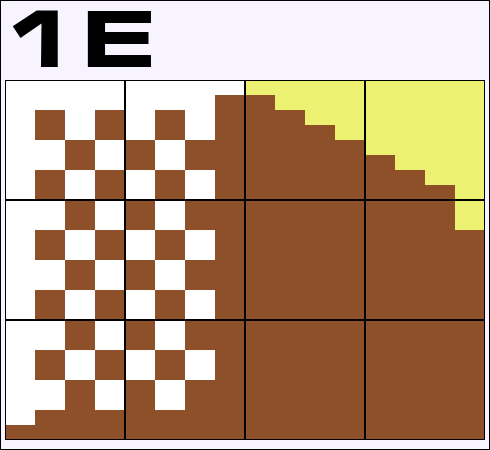
\includegraphics[height=3cm]{src/surface_structure_diagrams/6_1E_no_text.png}}
\hspace{0.4cm}
\raisebox{-0.1\totalheight}{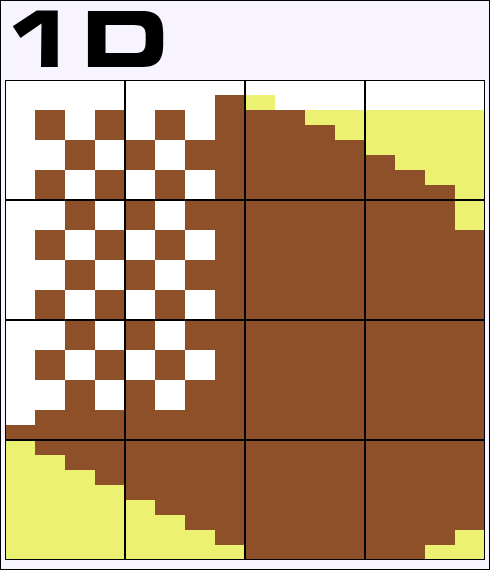
\includegraphics[height=3cm]{src/surface_structure_diagrams/6_1D_no_text.png}}
\hspace{0.4cm}
\raisebox{-0.1\totalheight}{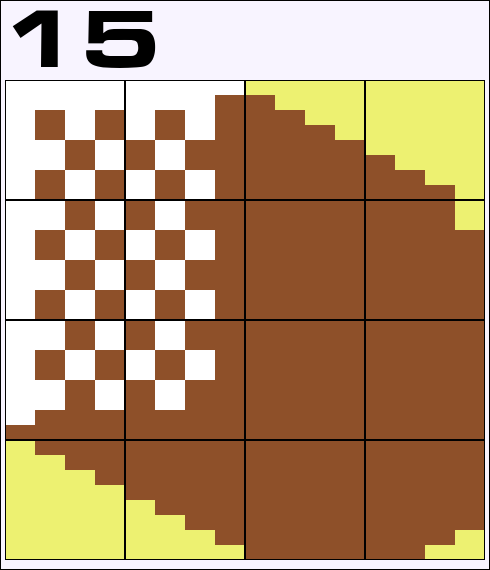
\includegraphics[height=3cm]{src/surface_structure_diagrams/6_15_no_text.png}}
\hspace{0.4cm}
\raisebox{-0.1\totalheight}{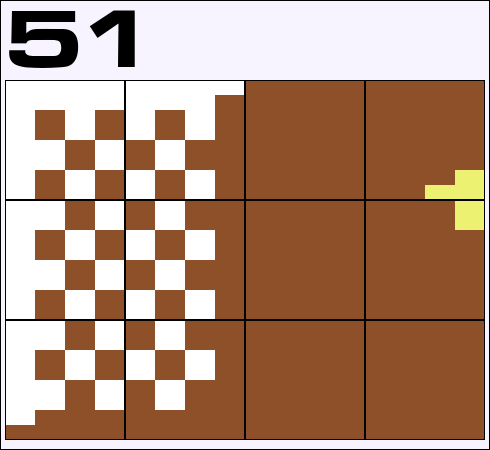
\includegraphics[height=3cm]{src/surface_structure_diagrams/6_51_no_text.png}}

This is what one of them, \icode{\$15}, looks like when replicated across a section creating a a diamond of plinths, along
with the data listing that tells us where to place each instance. Notice
that our "row numbers" are higher than in the previous diagram. This is because we are in the second half of the
ship, the second half of 256 bytes which make up the 512 bytes of each row in the ship in total.

\begin{minipage}[c]{0.72\linewidth}
\vspace{-0.5cm}
\begin{figure}[H]
    \begin{adjustbox}{width=10.2cm,left}
      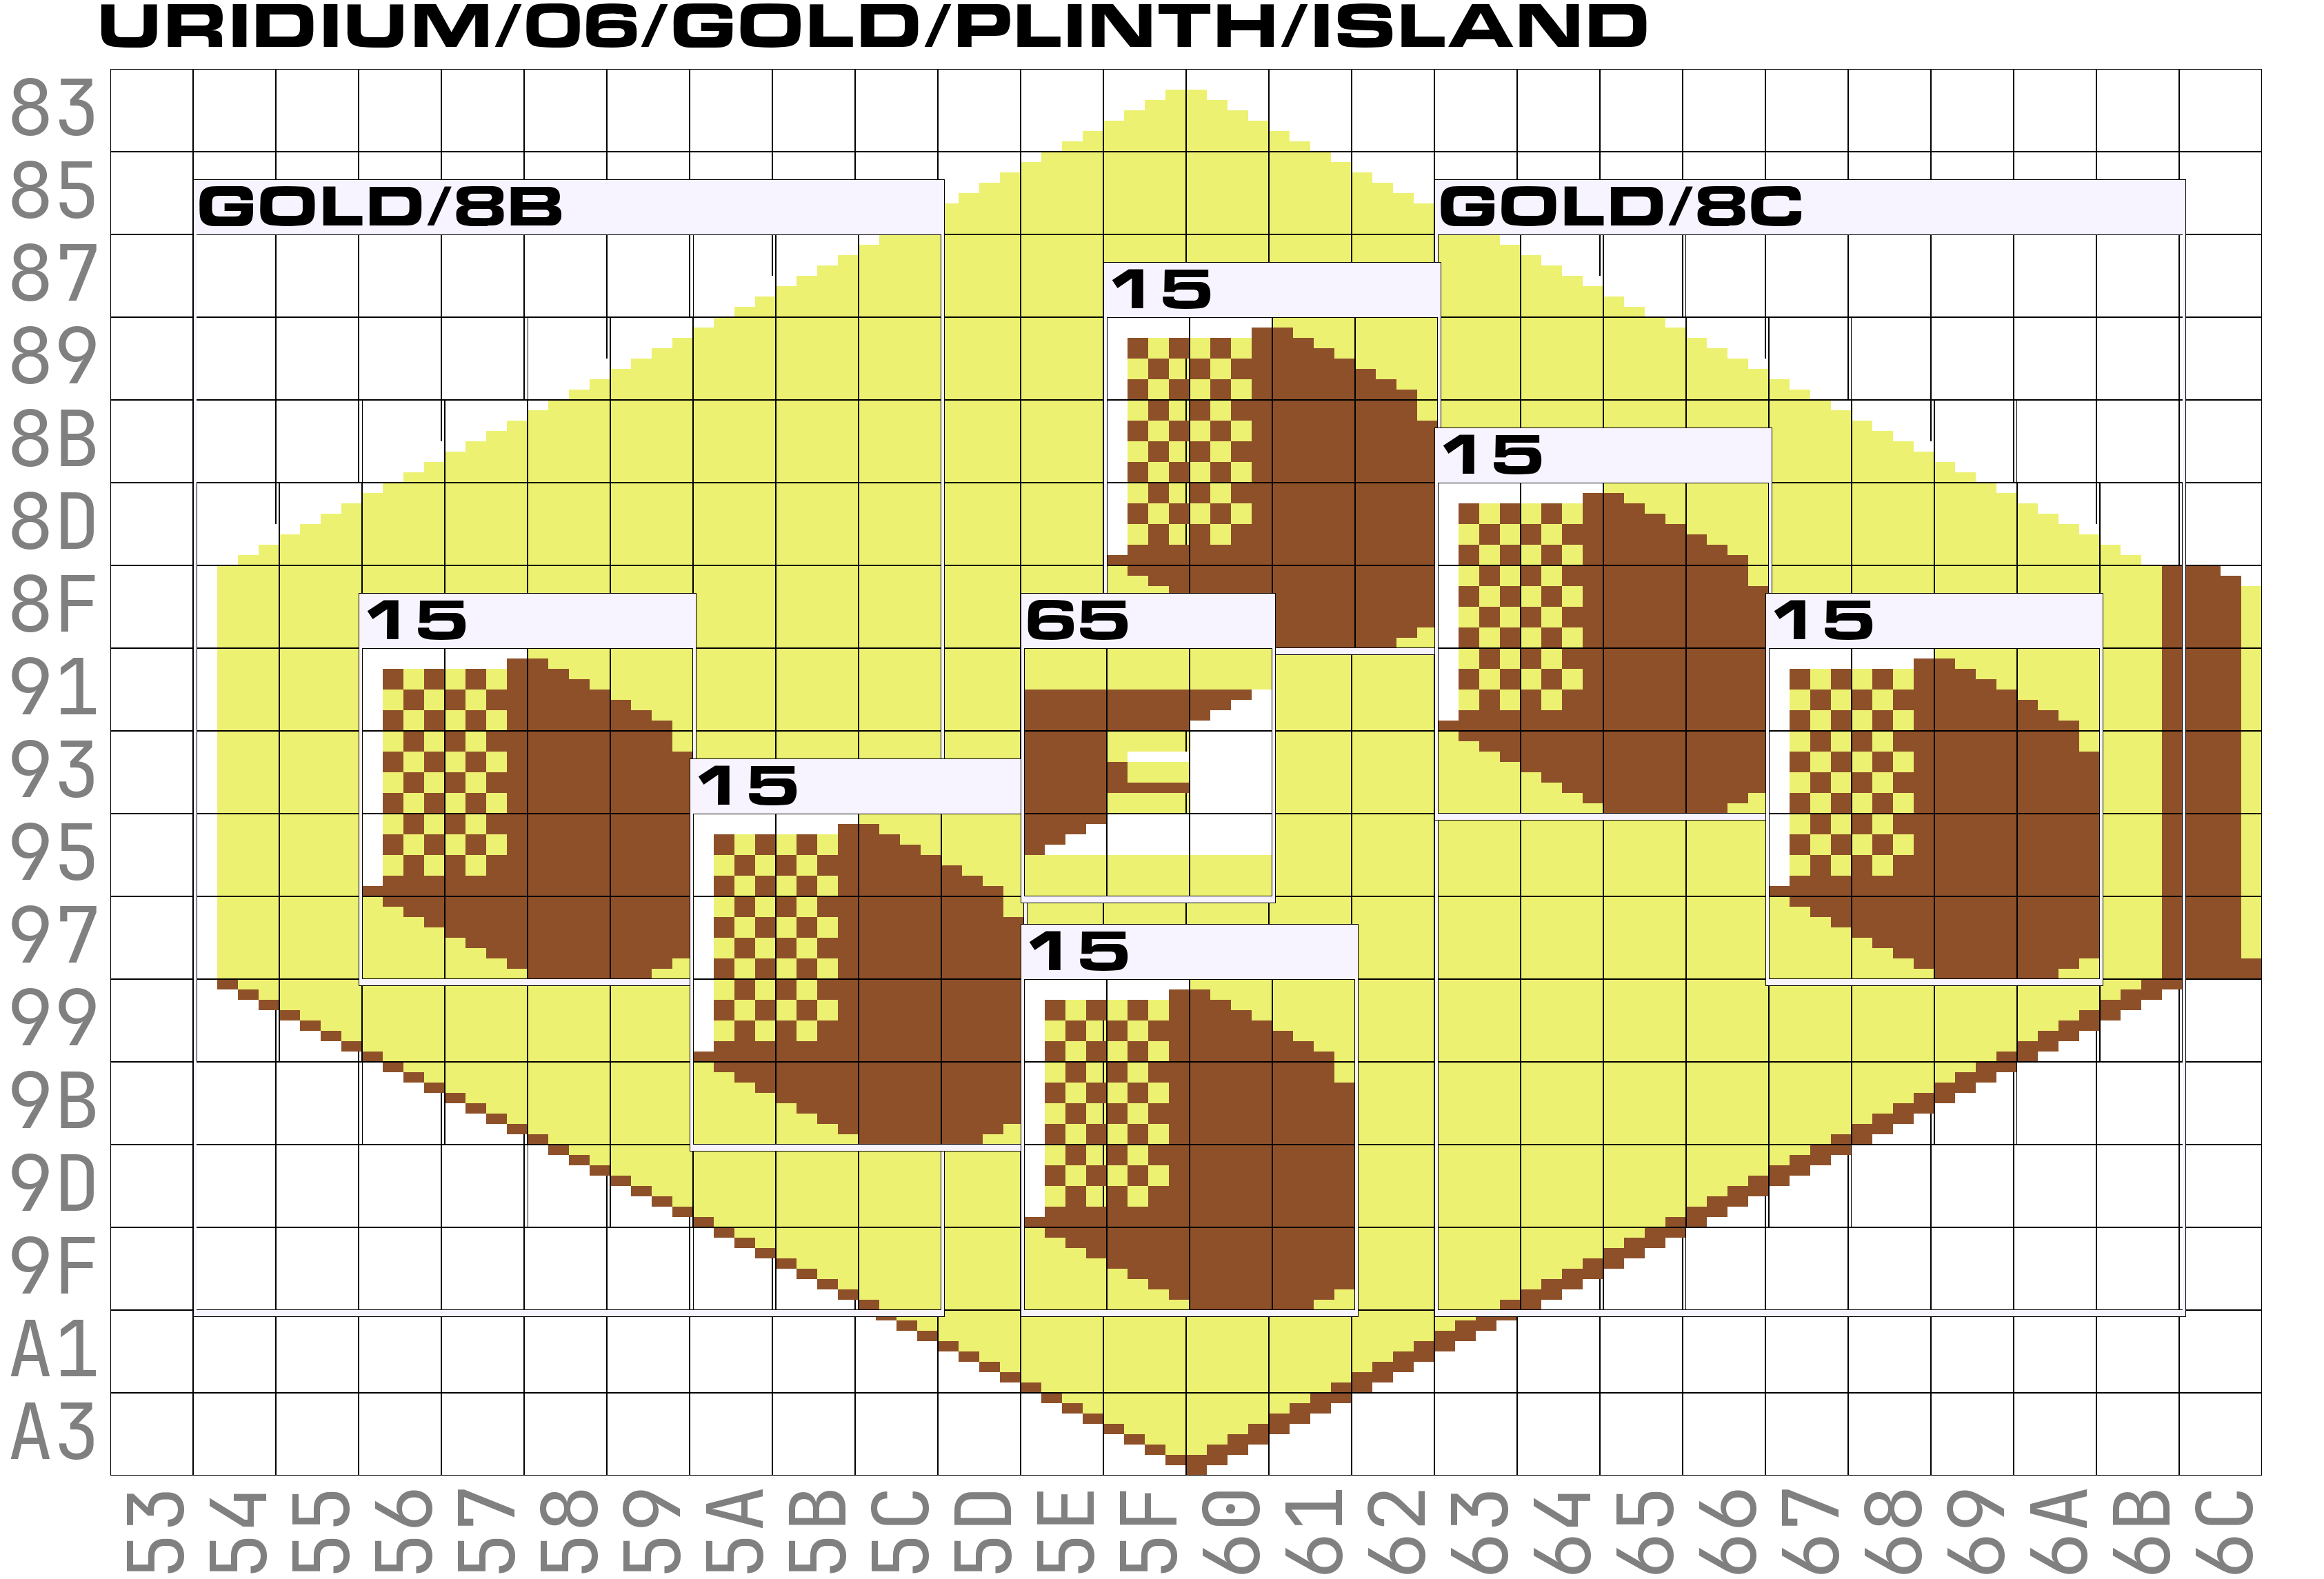
\includegraphics{src/surface_diagrams_with_sections/6_plinths.png}%
    \end{adjustbox}
\end{figure}
\end{minipage}
\hspace{0.6cm}
\begin{minipage}[c]{0.26\linewidth}
\begin{lstlisting}[basicstyle=\scriptsize\ttfamily]
.BYTE $97 ; High Byte
.BYTE $56 ; Low Byte 
.BYTE $15 ; Structure

.BYTE $9B ; High Byte
.BYTE $5A ; Low Byte 
.BYTE $15 ; Structure

.BYTE $9F ; High Byte
.BYTE $5E ; Low Byte 
.BYTE $15 ; Structure

.BYTE $8F ; High Byte
.BYTE $5F ; Low Byte 
.BYTE $15 ; Structure

.BYTE $93 ; High Byte
.BYTE $63 ; Low Byte 
.BYTE $15 ; Structure

.BYTE $97 ; High Byte
.BYTE $67 ; Low Byte 
.BYTE $15 ; Structure
\end{lstlisting}
\end{minipage}

There are bits of landing strip:

\raisebox{-0.1\totalheight}{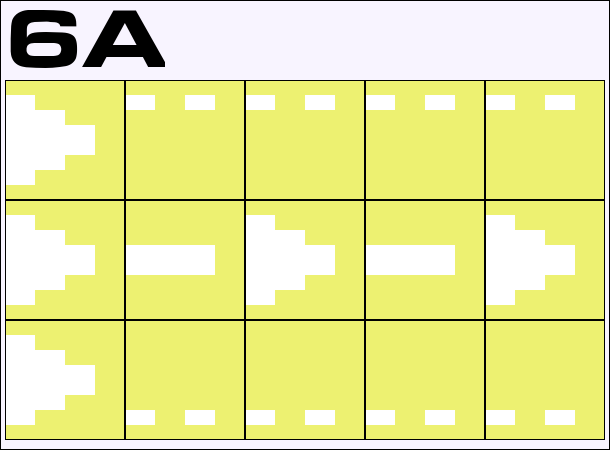
\includegraphics[height=3cm]{src/surface_structure_diagrams/6_6A_no_text.png}}
\hspace{0.4cm}
\raisebox{-0.1\totalheight}{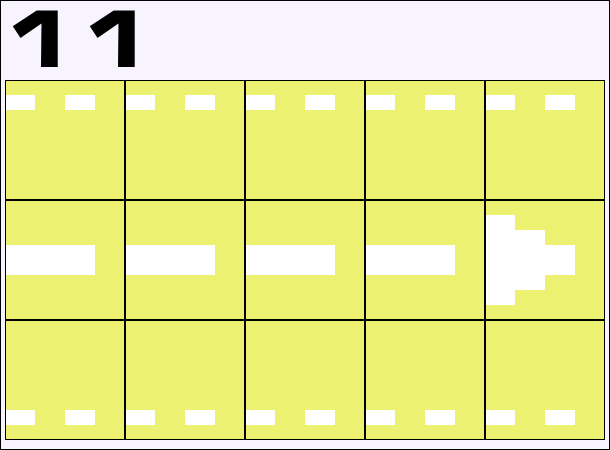
\includegraphics[height=3cm]{src/surface_structure_diagrams/6_11_no_text.png}}
\hspace{0.4cm}
\raisebox{-0.1\totalheight}{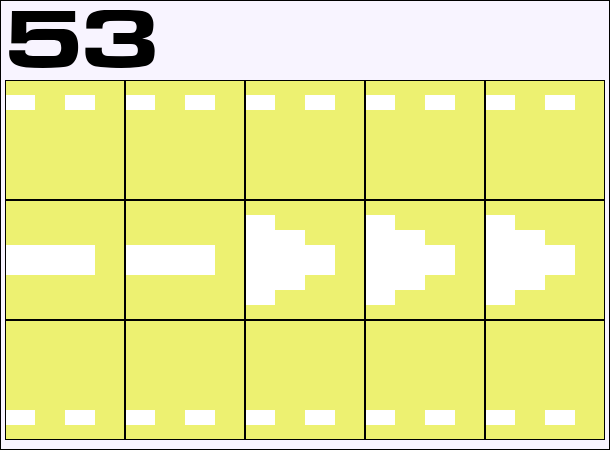
\includegraphics[height=3cm]{src/surface_structure_diagrams/6_53_no_text.png}}

And other interesting structures;

\raisebox{-0.1\totalheight}{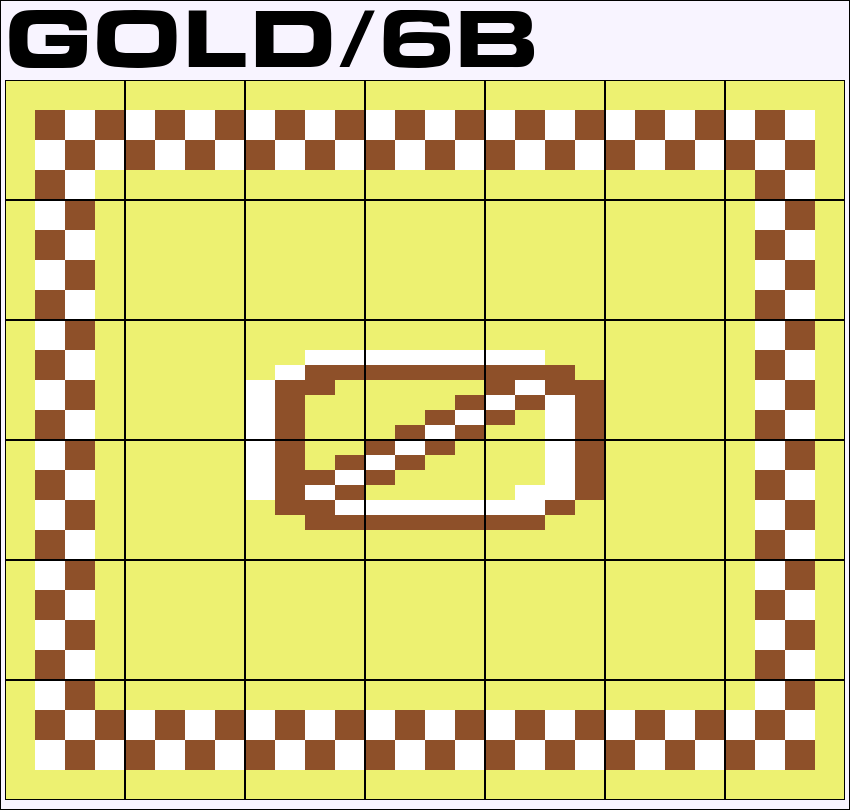
\includegraphics[height=3cm]{src/surface_structure_diagrams/6_6B_no_text.png}}
\hspace{0.4cm}
\raisebox{-0.1\totalheight}{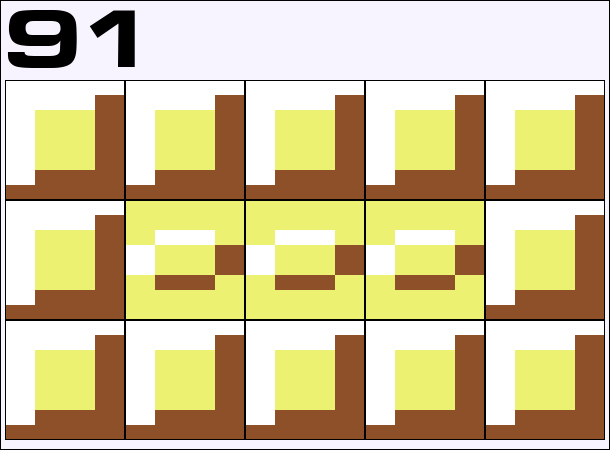
\includegraphics[height=3cm]{src/surface_structure_diagrams/6_91_no_text.png}}
\hspace{0.4cm}
\raisebox{-0.1\totalheight}{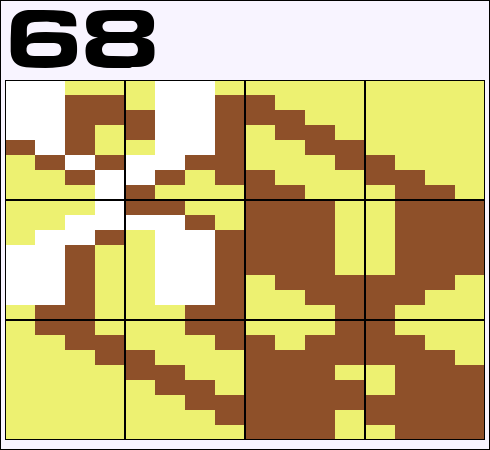
\includegraphics[height=3cm]{src/surface_structure_diagrams/6_68_no_text.png}}
\hspace{0.4cm}
\raisebox{-0.1\totalheight}{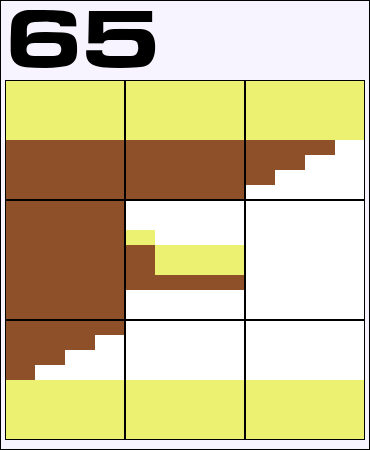
\includegraphics[height=3cm]{src/surface_structure_diagrams/6_65_no_text.png}}

By defining them as follows:

\begin{minipage}[c]{0.46\linewidth}
\begin{lstlisting}[basicstyle=\scriptsize\ttfamily]
.BYTE $8D ; High Byte (Row 6)
.BYTE $A4 ; Low Byte (Col 420)
.BYTE $11 ; Structure to Place

.BYTE $8D ; High Byte (Row 6)
.BYTE $A9 ; Low Byte (Col 425)
.BYTE $11 ; Structure to Place

.BYTE $8D ; High Byte (Row 6)
.BYTE $AE ; Low Byte (Col 430)
.BYTE $11 ; Structure to Place

.BYTE $8D ; High Byte (Row 6)
.BYTE $B3 ; Low Byte (Col 435)
.BYTE $11 ; Structure to Place

.BYTE $8D ; High Byte (Row 6)
.BYTE $B8 ; Low Byte (Col 440)
.BYTE $11 ; Structure to Place
\end{lstlisting}
\end{minipage}
\hspace{0.5cm}
\begin{minipage}[c]{0.46\linewidth}
\begin{lstlisting}[basicstyle=\scriptsize\ttfamily]
.BYTE $8D ; High Byte (Row 6)
.BYTE $BD ; Low Byte (Col 445)
.BYTE $53 ; Structure to Place

.BYTE $99 ; High Byte (Row 12)
.BYTE $9E ; Low Byte (Col 414)
.BYTE $68 ; Structure to Place

.BYTE $99 ; High Byte (Row 12)
.BYTE $A9 ; Low Byte (Col 425)
.BYTE $68 ; Structure to Place

.BYTE $99 ; High Byte (Row 12)
.BYTE $AF ; Low Byte (Col 431)
.BYTE $65 ; Structure to Place

.BYTE $99 ; High Byte (Row 12)
.BYTE $B8 ; Low Byte (Col 440)
.BYTE $91 ; Structure to Place
\end{lstlisting}
\end{minipage}


We can create this intriguing layout for the stern of the ship:

\begin{figure}[H]
    \begin{adjustbox}{width=14.2cm,left}
      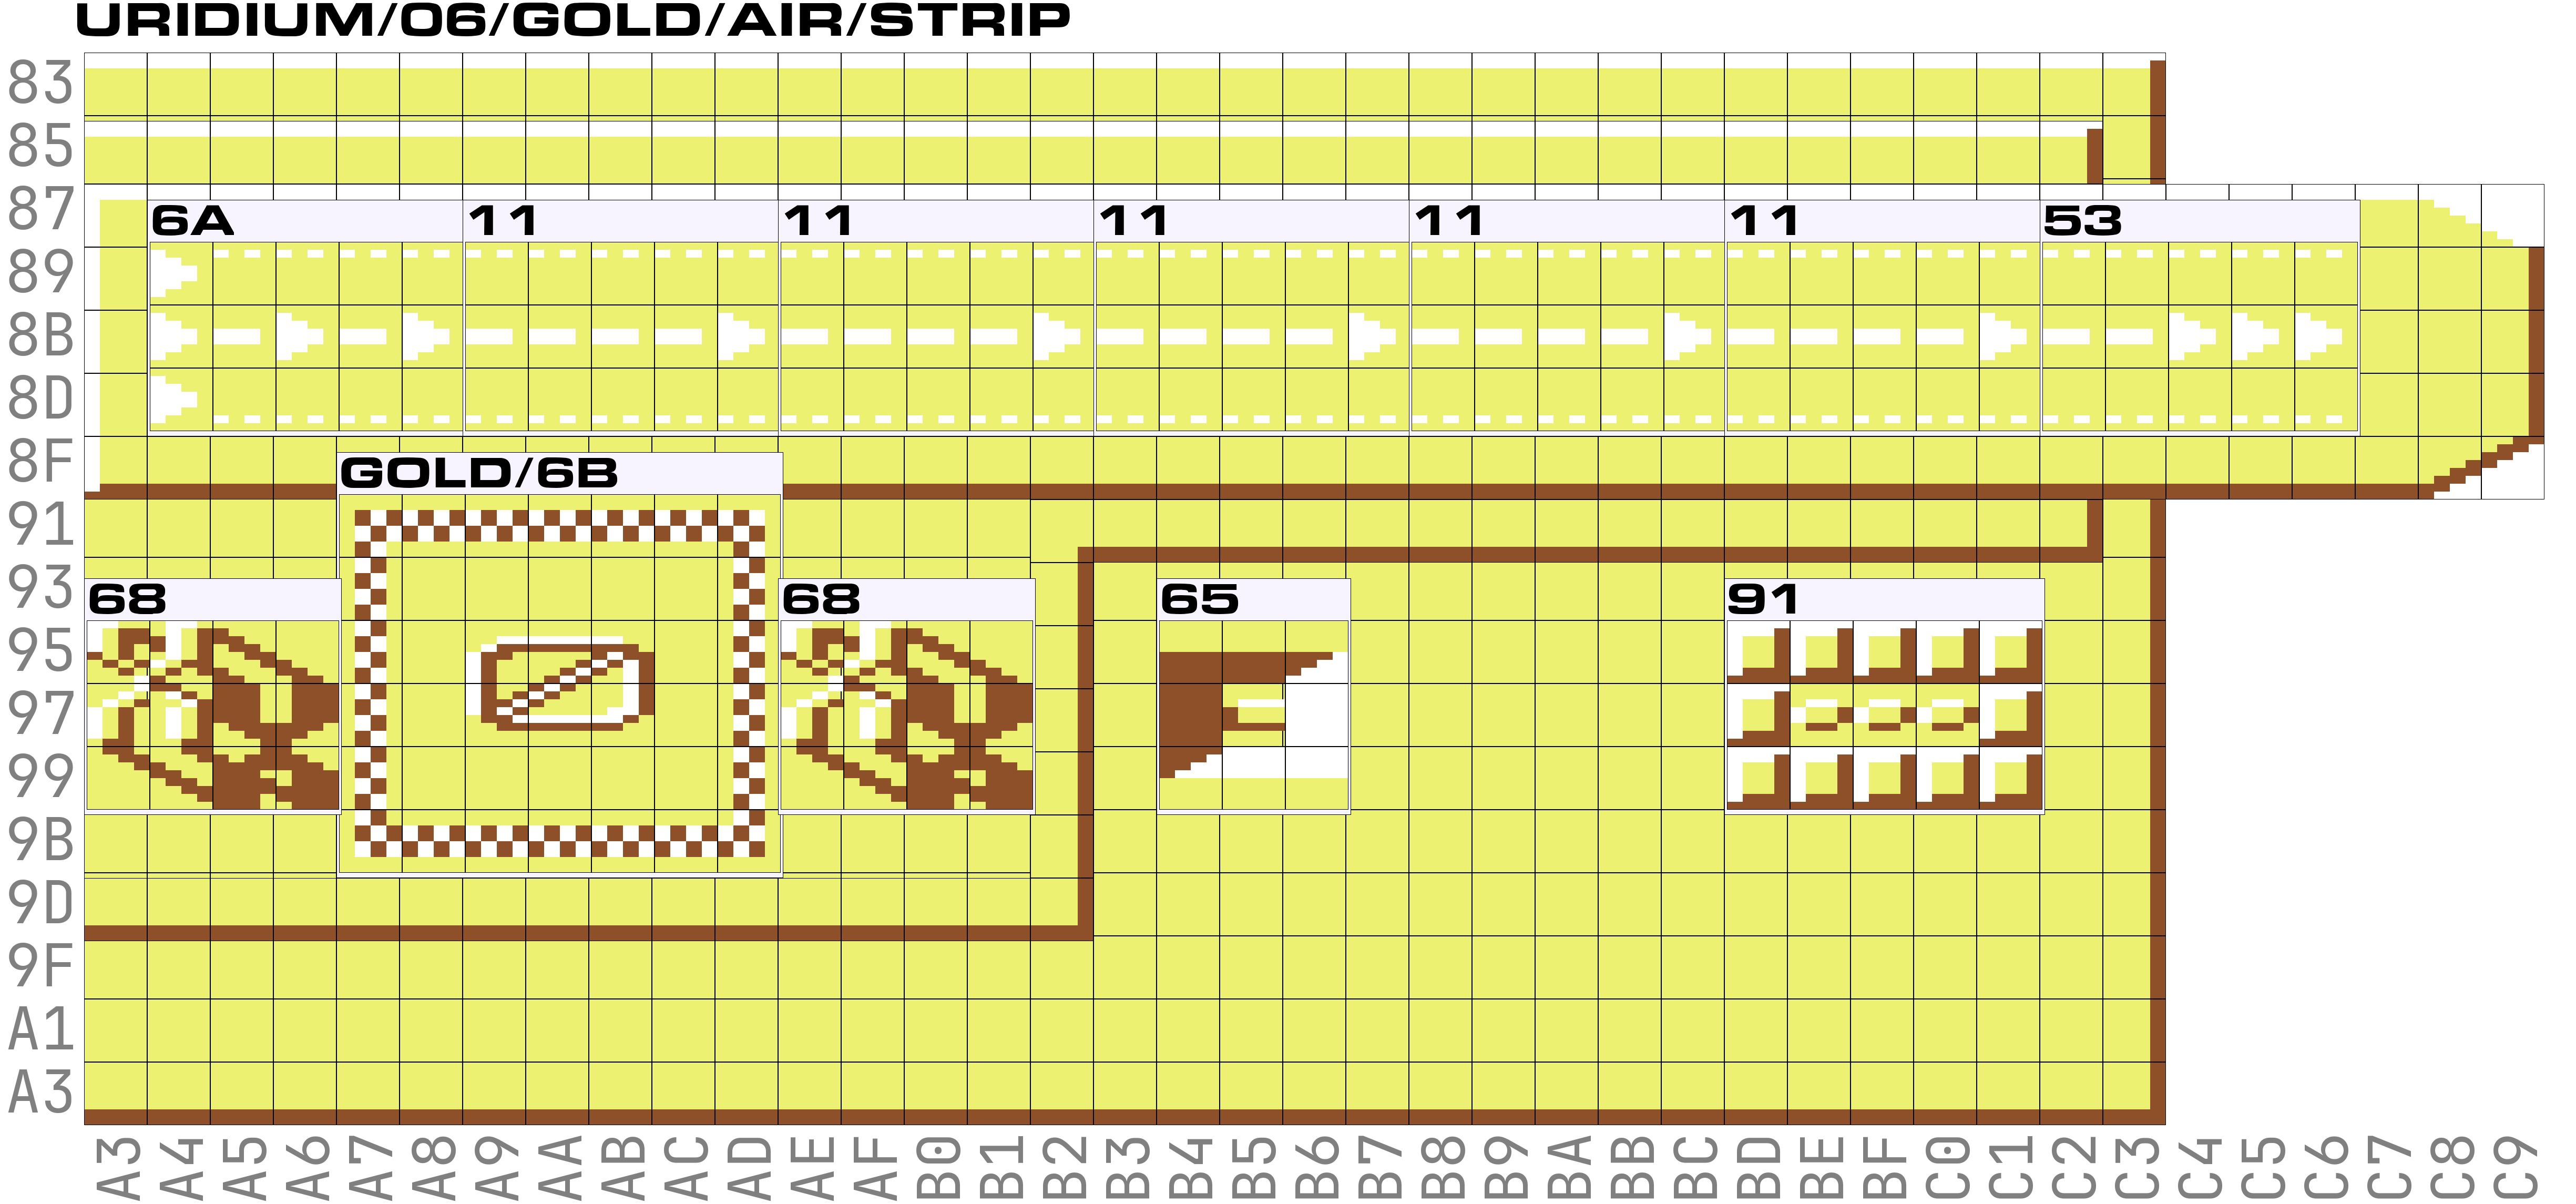
\includegraphics{src/surface_diagrams_with_sections/6_airstrip.png}%
    \end{adjustbox}
\end{figure}

There are bevelled squares of different sorts:

\raisebox{-0.1\totalheight}{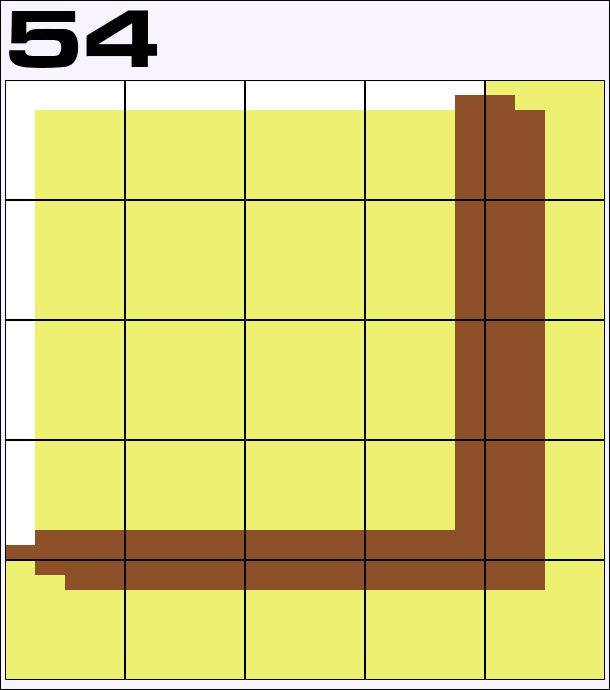
\includegraphics[height=3cm]{src/surface_structure_diagrams/6_54_no_text.png}}
\hspace{0.2cm}
\raisebox{-0.1\totalheight}{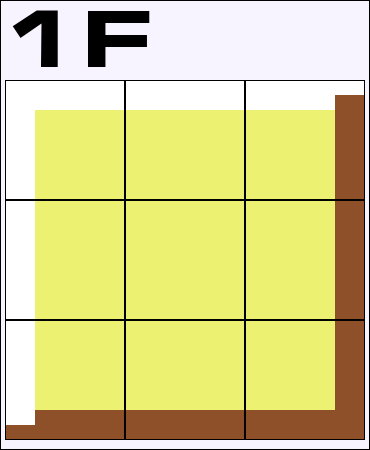
\includegraphics[height=3cm]{src/surface_structure_diagrams/6_1F_no_text.png}}
\hspace{0.2cm}
\raisebox{-0.1\totalheight}{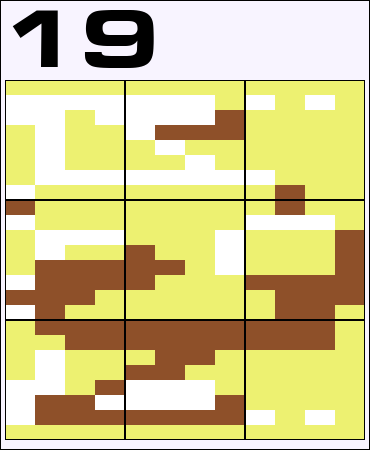
\includegraphics[height=3cm]{src/surface_structure_diagrams/6_19_no_text.png}}
\hspace{0.4cm}
\raisebox{-0.1\totalheight}{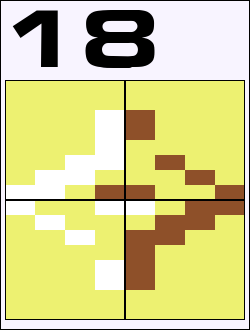
\includegraphics[height=3cm]{src/surface_structure_diagrams/6_18_no_text.png}}
\hspace{0.2cm}
\raisebox{-0.1\totalheight}{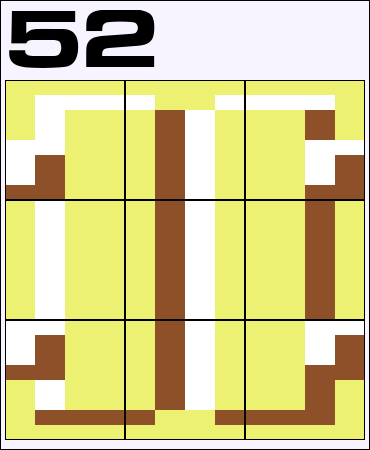
\includegraphics[height=3cm]{src/surface_structure_diagrams/6_52_no_text.png}}

We find these elements scattered around the surface, for example the air deck, rich in static aircraft (\icode{\$19}) waiting to be shot:

\begin{figure}[H]
    \begin{adjustbox}{width=14.2cm,left}
      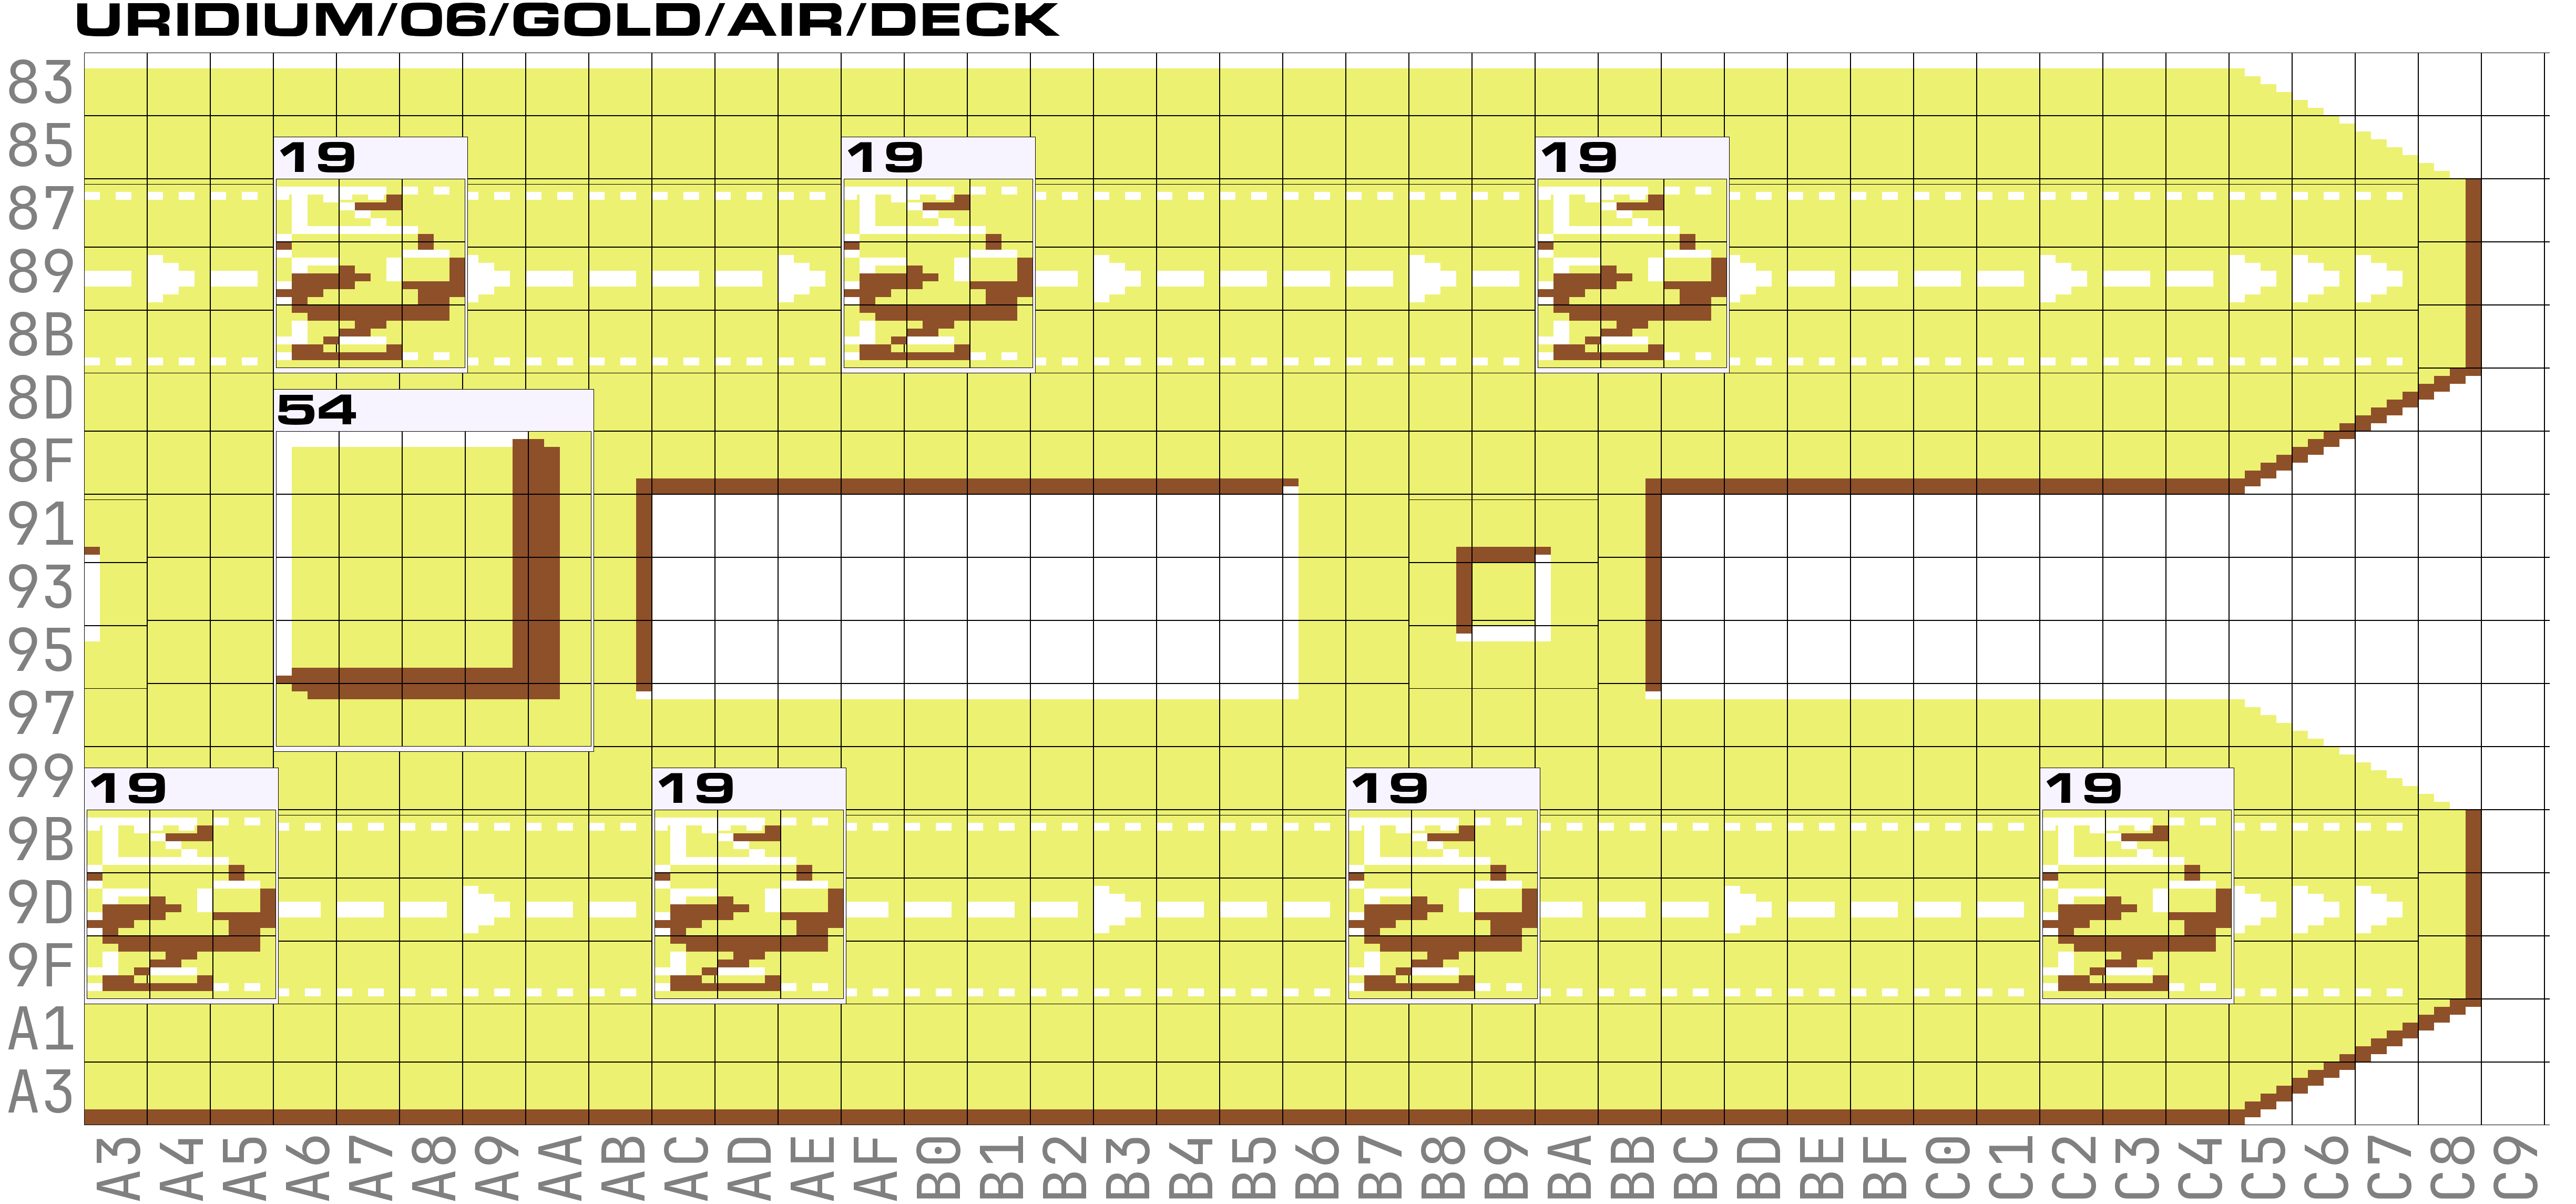
\includegraphics{src/surface_diagrams_with_sections/6_deck.png}%
    \end{adjustbox}
\end{figure}

To better understand the order in which the structures are drawn across the initially naked surface of the
dreadnought, we can take a look at the incremental progress observed in the 'Gold' level. We start with a completely
bare deck, containing no features, and even with some bow and stern sections missing:

\begin{figure}[H]
    \begin{adjustbox}{width=14cm,center}
      
\includegraphics{src/surfaces_raw_surface_only/6.png}%
    \end{adjustbox}
\end{figure}
\vspace{-0.6cm}

We notice that the first structures to be inserted complete the bow and stern detailing of the deck.
\begin{figure}[H]
    \begin{adjustbox}{width=14cm,center}
      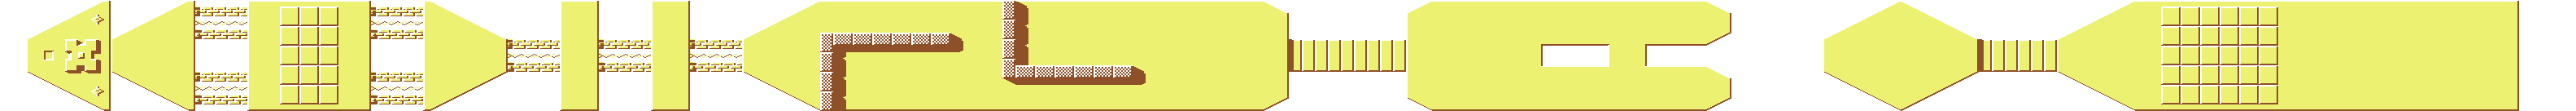
\includegraphics{src/surfaces_raw/6_progress_20.png}%
    \end{adjustbox}
\end{figure}
\vspace{-0.6cm}

Once those are in place, we see surface features in the bow section being added:
\begin{figure}[H]
    \begin{adjustbox}{width=14cm,center}
      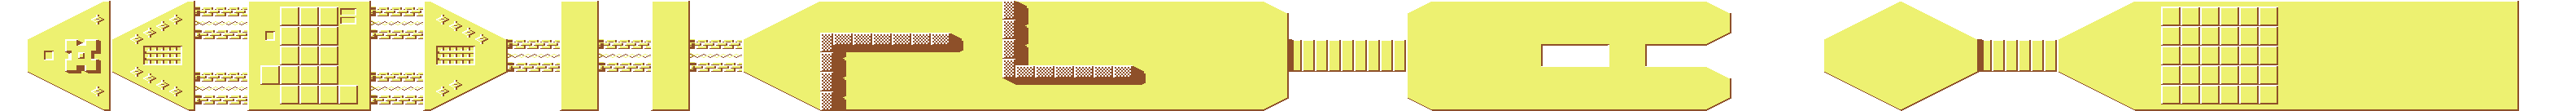
\includegraphics{src/surfaces_raw/6_progress_40.png}%
    \end{adjustbox}
\end{figure}
\vspace{-0.6cm}

The remaining structures are then added more or less in the order in which they appear on the surface, from 
left to right.

\begin{figure}[H]
    \begin{adjustbox}{width=14cm,center}
      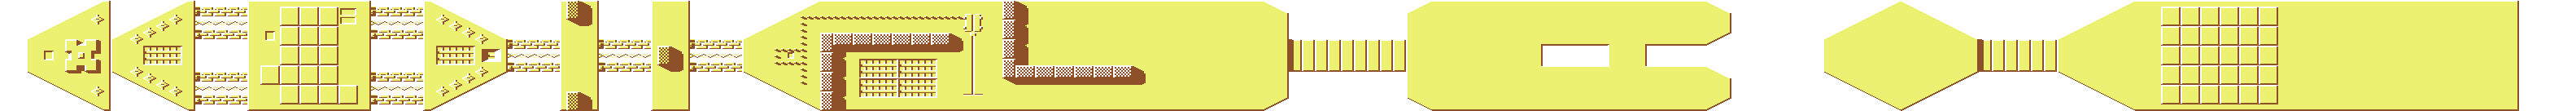
\includegraphics{src/surfaces_raw/6_progress_60.png}%
    \end{adjustbox}
\end{figure}
\vspace{-0.6cm}
\begin{figure}[H]
    \begin{adjustbox}{width=14cm,center}
      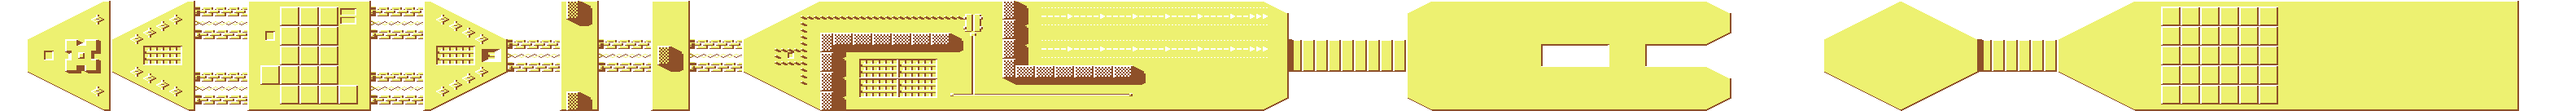
\includegraphics{src/surfaces_raw/6_progress_80.png}%
    \end{adjustbox}
\end{figure}
\vspace{-0.6cm}
\begin{figure}[H]
    \begin{adjustbox}{width=14cm,center}
      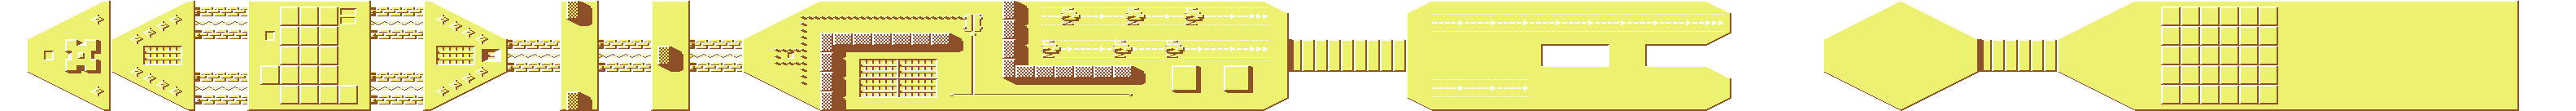
\includegraphics{src/surfaces_raw/6_progress_100.png}%
    \end{adjustbox}
\end{figure}
\vspace{-0.6cm}
\begin{figure}[H]
    \begin{adjustbox}{width=14cm,center}
      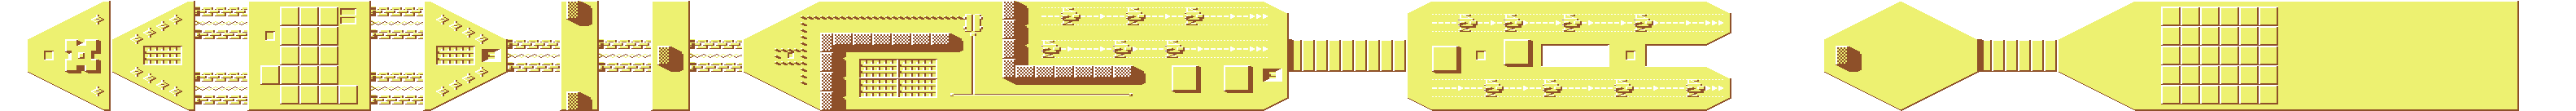
\includegraphics{src/surfaces_raw/6_progress_120.png}%
    \end{adjustbox}
\end{figure}
\vspace{-0.6cm}
\begin{figure}[H]
    \begin{adjustbox}{width=14cm,center}
      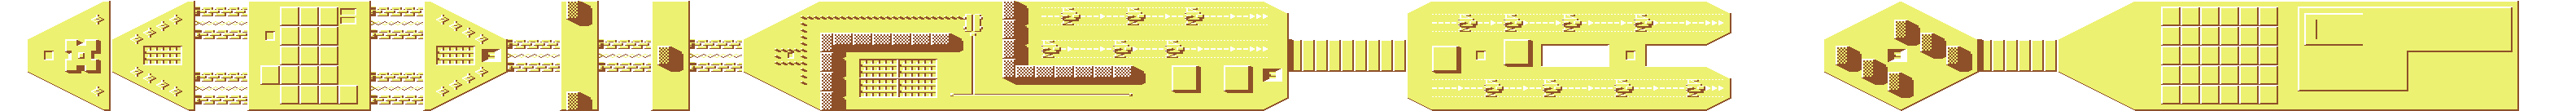
\includegraphics{src/surfaces_raw/6_progress_140.png}%
    \end{adjustbox}
\end{figure}
\vspace{-0.6cm}

Finally the entire dreadnought is complete. 
\begin{figure}[H]
    \begin{adjustbox}{width=14cm,center}
      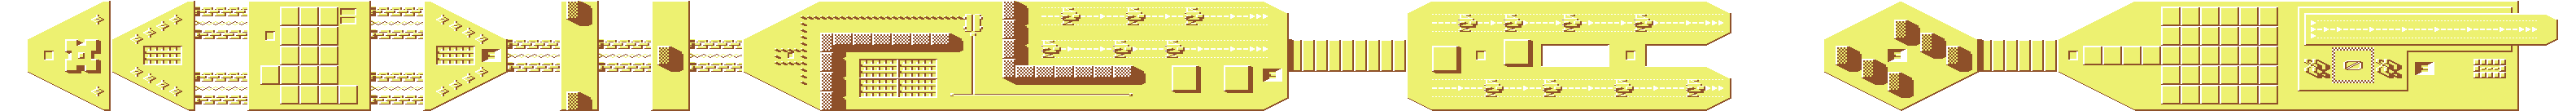
\includegraphics{src/surfaces_raw/6.png}%
    \end{adjustbox}
\end{figure}
\vspace{-0.6cm}
With this in mind, we can take some time to carefully read the routine (opposite)
that performs this activity. We observe how the inner loop \icode{DrawStructure} is responsible
for consuming and rendering the data for each specified structure, while the outer loop \icode{DrawPlacedStructures}
manages the business of reading in the list of structures to render. Notice how at the start we read in the byte-pair address
for placing the structure and then the index of the structure data that we must use. These are the three bytes we mentioned
earlier that each consitute a single entry in the full list of structures for placement on the surface of the dreadnought. 

\clearpage
\begin{lstlisting}[basicstyle=\scriptsize\ttfamily]
DrawPlacedStructures   
  ; Get the address in surface data at which to draw the structure.
  LDA (dreadnoughtDataLoPtr),Y ; Read in the High Pointer Byte
  STA levelSurfaceHiPtr        ; Store it.
  CMP #>endOfSurfaceData       ; Have we reached the end yet?
  BCS FinishSurfaceAndReturn   ; If so, we've finished drawing structures.

  INY                          ; Move our pointer to the next byte in the data.
  LDA (dreadnoughtDataLoPtr),Y ; Read in the Low Pointer Byte
  STA levelSurfaceLoPtr        ; Store it.

  ; Get the index for the structure to draw and the structure data referenced by it.
  INY                          ; Move our pointer to the next byte in the data.
  LDA (dreadnoughtDataLoPtr),Y ; Read in the structure index.
  BEQ FinishSurfaceAndReturn   ; If it's a $00 then we're finished.
  TAX                          ; Transfer the index to X.
  LDA surfaceStructureDataHiPtrArray,X ; Get the High Byte of the structure data.
  STA structureDataHiPtr       ; Store it.
  LDA surfaceStructureDataLoPtrArray,X ; Get the Low Byte of the structure data.
  STA structureDataLoPtr       ; Store it.

  ; Move index forward 3 bytes to the next address and structure (for later).
  LDA dreadnoughtDataLoPtr     ; Get the current pointer.
  ADC #$03                     ; Increment it by 3.
  STA dreadnoughtDataLoPtr     ; Store it.

  ; The start of each structure data contains the number of strips in the section.
  LDY #$00
  LDA (structureDataLoPtr),Y   ; Read number of strips in to 'A'.
  INY                          ; Move our pointer to the next byte in the data.
  STA numberOfStrips           ; Store the number of strips.

  ; Draw each strip of the structure.
DrawStructure   
  LDA (sectionDataLoPtr),Y     ; Read in the length of the strip.
  INY                          ; Move index to next position.
  TAX                          ; Store the length in X.
ProcessCharacterInStrip   
  LDA (structureDataLoPtr),Y   ; Get a charset value from the section and store in A.
  INY                          ; Increment our pointer to the data.
  STY stashedYValue            ; Stash it.
  LDY #$00                     ; Use Y as a pointer to the surface. 
  CMP #SPACE                   ; Is the character a 'blank space'?
  BEQ Continue                 ; If so, don't write it..
  STA (levelSurfaceLoPtr),Y    ; Otherwise write the tile to the screen.
Continue   
  LDY stashedYValue            ; Restore Y.
  DEC levelSurfaceHiPtr        ; Move up to the next char in the strip (512 bytes) ..
  DEC levelSurfaceHiPtr        ; .. by decrementing the high pointer twice.
  BPL FinishSurfaceAndReturn   ; Exit if we've reached the end.
  DEX                          ; Otherwise move to the next character.
  BNE ProcessCharacterInStrip  ; And process it.
  ; Go to the next strip
  LDA levelSurfaceLoPtr        ; Get position of current strip on dreadnought.
  ADC #$01                     ; Increment by one in order to draw ..
  STA levelSurfaceLoPtr        ; .. the next strip in the next position to the right.
  DEC numberOfStrips           ; Otherwise, do the next strip in the section.
  BNE DrawStructure       ; Keep looping until all strips in the section are done.

  ; Go to the next substructure.
  LDY #$00                     ; Set Y to 0.
  JMP DrawPlacedStructures     ; Draw the next structure.
\end{lstlisting}

